\documentclass[12pt]{article}
\usepackage{amsmath,amsthm}
\usepackage[utf8]{inputenc}
%\usepackage[T1]{fontenc}
%\usepackage{minionpro}
\usepackage{array,graphicx}
\usepackage{chicago}        %bibliography style
\usepackage{booktabs}       %to make table lines thicker

\setlength{\topmargin}{-0.3in} \setlength{\textheight}{8.75in}
\setlength{\oddsidemargin}{0.25in} \setlength{\evensidemargin}{0.25in}
\setlength{\textwidth}{6in}
\def\labelenumi{\arabic{enumi}.}
\def\theenumi{\arabic{enumi}}
\def\labelenumii{(\alph{enumii})}
\def\theenumii{\alph{enumii}}
\def\p@enumii{\theenumi.}
\def\labelenumiii{\arabic{enumiii}.}
\def\theenumiii{\arabic{enumiii}}
\def\p@enumiii{(\theenumi)(\theenumii)}
\def\labelenumiv{\arabic{enumiv}.}
\def\theenumiv{\arabic{enumiv}}
\def\p@enumiv{\p@enumiii.\theenumiii}
\pagestyle{plain}
\pagestyle{plain} \setcounter{secnumdepth}{3}
\newcommand{\D}{\mathop{\mathrm{d\mathstrut}}\nolimits\!}
\newcommand{\dt}{\D t}
\newcommand{\dz}{\D z}
\newcommand{\E}{\mathop{\mathrm{E\mathstrut}}\nolimits}
\newcommand{\Var}{\mathop{\mathrm{Var\mathstrut}}\nolimits}
\newcommand{\sd}{\mathop{\mathrm{sd\mathstrut}}\nolimits}
\newcommand{\diag}{\mathop{\mathrm{diag\mathstrut}}\nolimits}
\newcommand{\Cov}{\mathop{\mathrm{Cov\mathstrut}}\nolimits}
\newcommand{\Corr}{\mathop{\mathrm{Corr\mathstrut}}\nolimits}
\newtheorem{definition}{Definition}
\newtheorem{proposition}{Proposition}
\newtheorem{conjecture}{Conjecture}
\newtheorem{moment}{Empirical regularity}
\newtheorem{insight}{Qualitative prediction}

\renewcommand{\baselinestretch}{1.17}

\newcommand{\dofigure}[3]{\begin{figure}
\begin{centering}
\includegraphics[width=0.75\linewidth]{figures/#1}
  \caption{#2\label{fig:#1}}
\end{centering}

\noindent \footnotesize{#3}
\end{figure}}

\newcommand{\dotable}[2]{\begin{table}[h!]
\begin{centering}
\caption{#2\label{tab:#1}}
\includegraphics[width=0.75\linewidth]{figures/#1}
\end{centering}
\end{table}}

\begin{document}

\title{Cattle, Steaks and Restaurants:\\ Development Accounting when Space Matters\thanks{For useful comments, we thank Thomas Holmes, Esteban Rossi-Hansberg, Albert Saiz, Adam Szeidl, Jonathan Vogel, Kei-Mu Yi and audiences of the Conference on Urban and Regional Economics and seminars at Central European University, Princeton University and the Philadelphia Fed.}}
\author{Péter Karádi\thanks{European Central Bank. E-mail: peter.karadi@ecb.int} and Miklós Koren\thanks{Central European University, IE-CERS and CEPR. E-mail: korenm@ceu.hu.}}
\maketitle

\begin{abstract}
We conduct sector-level development accounting in a macro model where land and location play a role. Producers in agriculture, manufacturing and services choose their location to trade off transport costs to the city center and rents. We solve for the spatial equilibrium and show how space affects the aggregate production function and measured productivity. Studies not accounting for sector location will deem services in large, expensive cities unproductive. This biases development accounting because rich countries have large service-cities. Our preliminary calibrations show that, correcting for sector location, service productivity varies as much across countries as manufacturing productivity does. This is in contrast with previous studies that found smaller variation in service productivity.
\end{abstract}

Productivity is much lower in poor countries than in rich ones (\citeN{Klenow97}, \citeN{Hall99}, \citeN{Caselli05}). To understand the fundamental causes of productivity differences, it is important to identify the sectors in which these differences are the greatest. Several recent papers have studied the sectoral composition of productivity differences by using data on sector-level inputs, outputs and prices (\citeN{Bailey01}, \citeN{Caselli05}, \citeN{Duarte10}, \citeN{Restuccia08}). Their main result is that productivity differences are sizeable and they are larger in agriculture than in manufacturing and services.\footnote{These results are in line with the classic Balassa-Samuelson literature (\citeN{Balassa64}, \citeN{Samuelson64}, \citeN{Baumol65}, \citeN{Baumol67}), which explains sectoral price-level differences by productivity advantage of manufacturing over services.} 

Productivity estimation is always contingent on the set of inputs included in the production function and their quality. Unobserved variation in the quantity or quality of inputs will necessarily show up as variation in productivity. Here we argue that land input has been conspicously (?) missing from development accounting exercises to date.

Controlling for land when estimating macro productivity is important for two reasons. First, countries with high population density are relatively scarce in land and, to the extent that land matters in production, these countries will be deemed less productive. Second, land varies in a crucial quality component: its proximity to consumers. Urban land is more valuable because it is more productive in producing XX. Again, countries may differ in the availability of urban land, thus biasing productivity estimates.

Accounting for land and location is especially important for sector-level development accounting. Agriculture uses land intensively and will be especially sensitive to controlling for the quantity of land. Services, in turn, locate in urban areas and will be especially sensitive to controlling for location. XX RELEVANCE

We build a simple multi-sector general equilibrium model. Each sector uses labor (or a composite of other spatially mobile inputs) and land. The location of sectors is determined in the canonical von Thünen city model. In the model, all trade happens in the city center, the central business district (CBD). Producers choose their location freely on a plane, and have to pay a shipping cost to transport their goods to the CBD. This spatial structure introduces variable land-quality to the model, as land closer to the CBD saves on transport cost. Equilibrium rents decrease with distance from the CBD, and the producers optimally choose locations to balance savings on transport costs to higher rents.
%The valuation of the land-quality is sector-specific: sectors with the highest shipping costs and lowest land intensity value location the most. XXX ANYTHING ELSE?
Our model yields a simple spatial equilibrium in which agriculture (``cattle'') locates farthest away from the center, manufacturing (``steaks'') occupies a ring outside the center, and services (``restaurants'') are in a central circle.

There are two reasons why development accounting in our model is different from models without land. First, as some sectors are more land intensive, their prices may be more sensitive to rents. Because of this, conditional on productivity, agricultural prices will be relatively higher in rich countries. Second, because sectors endogenously choose locations, their price is also affected by the rent gradient: the speed with which rents decline in distance from the city center. Urban sectors will be relatively more expensive in countries where the rent gradient is higher (larger, more service-intensive, more urbanized countries).

To quantify the importance of these two mechanisms, we calibrate our model in a set of developed and emerging-market countries with comparable data on sector level productivites and prices.\footnote{We are using the EUKLEMS database, see \citeN{OMahony09}.} We set common technology parameters to match the sectoral land-shares and spatial distribution of economic activities in the U.S., and allow international variation in the level of urbanization and sector-shares of output. We then use the calibrated model to infer location-corrected sector-level productivities for each country. Our main question is whether explicitly controlling for endogenous location choice has the potential to change previous quantitative conclusions on sectoral productivity differences. %(XX AND URBANIZATION)

XX RESULTS

\bigskip

Beyond the development accounting papers cited above, our work is related to MACRO URBAN


\section{Motivating facts}
1. The rent gradient increases with development. Urban land becomes more important both in absolute terms and relatively. (Clark, 2007)
2. The relative price of services increase with development. Baumol's cost disease.
3. Rich countries are more urbanized.
4. Rich countries produce less agriculture and more services.


\section{A model of industry location}
We introduce location choice to a multi-sector general equilibrium model. We have three sectors: agriculture, manufacturing and services, each using land and labor for production. Our spatial structure follows the von Thünen monocentric city model: producers choose a location on the plane and need to transport their goods to the central business district. %They differ in the land intensity of their production (significantly higher with agriculture) and their transport costs (significantly higher with services).

\subsection{Consumers}
Consumers have Cobb--Douglas preferences across goods produced by the three sectors,
\begin{equation}
\label{eq:Utility}
U = C_1^{\alpha_1}C_2^{\alpha_2}C_3^{\alpha_3},
\end{equation}
with $\sum_{i=1}^3\alpha_i=1$. They supply labor $N$ inelastically, and rent land to producers in a competitive market. They are \emph{absentee landlords}: the rents they collect are independent of the place of employment.

%% make this nonhomogeneous

Their budget constraint is
\begin{equation}
\label{eq:BudCons}
PC=WN+\int_z R(z)\tilde{L}(z)dz,
\end{equation}
where $C=\Pi_{i=1}^3C_i^{\alpha_i}$ and $P=\Pi_{i=1}^3P_i^{\alpha_i}/\Pi_{i=1}^3\alpha_i^{\alpha_i}$ are the quantity and price of the composite good, respectively. $R(z)$ is the rent as a function of the distance to the center (see later), and $W$ is the wage. Because labor is freely mobile, wages do not depend on location.

The parameters $\alpha_i$ determine the sectoral consumption shares:
\begin{equation*}
\alpha_i=\frac{P_iC_i}{PC}.
\end{equation*}

\subsection{Producers}
\subsubsection{Technology}
Output in sector $i$ at location $z$ depends on employment $N$ and land $L$ used at that location,
\[
Q_i(z) = A_i L_i(z)^{\beta_i}N_i(z)^{1-\beta_i}.
\]
We take labor to be freely mobile within the country, land is in fixed $\tilde{L}(z)$ supply in each location. The names ``land'' and ``labor'' are for the sake of convenience, these two factors correspond to spatially fixed and mobile factors, respectively, and we will calibrate them accordingly.

Sectors differ in their land shares $\beta_i$ and Hicks neutral productivity shifter $A_i$.

All products are sold and consumed at a single location, the central business district. This is location $z=0$, so that $z$ indexes distance to the center.

\subsubsection{Shipping}
To ship a product to the center, one has to incur shipping costs. If a unit of product $i$ leaves location $z$, only
\[
e^{-\tau_i z}
\]
units arrive at the center. This is akin to the iceberg assumption of transport costs. Sectors also differ in the intensity of shipping costs $\tau_i$.

\subsubsection{Profits}
Profits in sector $i$ from production at $z$ is
\begin{equation}
\label{eq:profit}
\Pi_i(z)=P_ie^{-\tau_iz}Q_i(z)-WN_i(z)-R(z)L_i(z).
\end{equation}
A sector being active at location $z$ requires that their maximized profit $\max\Pi_i(z)\geq0.$

\subsection{Single-city Equilibrium}
We begin by characterizing the equilibrium of a single city with fixed amount of land and labor.

The competitive spatial equilibrium in a circular city $z\in Z$ is an equilibrium set of quantities $\{C_i, Q_i(z), L_i(z), N_i(z)\}_{i=1}^3$ and prices $\{P_i, R(z), W\}_{i=1}^3$ such that
\begin{enumerate}
    \item The consumer chooses $\{C_i\}_{i=1}^3$ to maximize utility (\ref{eq:Utility}) subject to its budget constraint (\ref{eq:BudCons}), taking prices as given.
    \item The producers choose technology $i$ and location $z$, and nonnegative quantities $\{Q_i(z), L_i(z), N_i(z)\}$ to maximize their profits (\ref{eq:profit}), taking prices as given.
    \item Sectoral goods market clear: $C_i=\int_{z\in Z} e^{-\tau_iz}Q_i(z)dz$ for $i=1,2,3$.
    \item Labor market clears: $N=\sum_i\int_{z\in Z} N_i(z)$.
    \item Land markets clear at every location: $\sum_iL_i(z)=\tilde L(z)$ for all $z\in Z$.
\end{enumerate}

\subsection{Spatial structure}
The equilibrium, as we show below, has a simple and intuitive structure. Sectors with higher transport cost intensity ($\tau_i$) and lower land share ($\beta_i$) locate closer to the center. Realistically, services locate in a circle around the center, manufacturing goods are produced on a ring around it, and agriculture inhibits the outer ring.

To see why it is the case, it is instructive to construct the sectoral bid rent curves $R_i(z)$. These are the maximum rent an active producer with technology $i$ would be willing to pay at location $z$. %In a competitive market, the sector with the highest bid rent curve is active at a location ($R(z)=\max_iR_i(z)$ for all $z$).
A profit maximizing producer is choosing its land $N_i(z)$ and labor demand $L_i(z)$ to equalize the value marginal product of land and labor to rents and wages, respectively. It is true for any rent function or wages it might face, so it is true for rents given by its own bid-rent curve $R_i(z)$, in particular.
\begin{align}
R_i(z) &=\beta_i P_ie^{-\tau_i z}A_i \left(\frac{N_i(z)}{L_i(z)}\right)^{1-\beta_i}\\
W &=(1-\beta_i) P_ie^{-\tau_i z}A_i \left(\frac{N_i(z)}{L_i(z)}\right)^{-\beta_i}
\end{align}

The sectoral labor-land ratio (employment density) can be expressed as
\begin{equation}
\label{eq:EmpDens}
\frac{N_i(z)}{L_i(z)} = \frac{1-\beta_i}{\beta_i}\frac{R_i(z)}{W}.
\end{equation}
Substituting this into the FOC for land, we can get an implicit expression for the sectoral bid rent curve:
\[
R_i(z) =\beta_i P_ie^{-\tau_i z}A_i \left(\frac{1-\beta_i}{\beta_i}\frac{R_i(z)}{W}\right)^{1-\beta_i},
\]
%\[
%R_i(z)^{\beta_i} =\beta_i^{\beta_i}(1-\beta_i)^{1-\beta_i} P_ie^{-\tau_i z}A_i W^{\beta_i-1}
%\]
from which
\begin{equation}
\label{eq:BidRent}
R_i(z) =\beta_i(1-\beta_i)^{1/\beta_i-1} (P_iA_i)^{1/\beta_i} W^{1-1/\beta_i} e^{-\frac{\tau_i}{\beta_i} z}.
\end{equation}
Equation (\ref{eq:BidRent}) pins down the gradient of the sectoral rent curve, which determines how fast the bid-rents decrease with the distance from the CBD. The gradient is an increasing function of the sectoral transport costs and a decreasing function of land shares $|\partial\log R_i(z)/\partial \log z|=\tau_i/\beta_i$. Intuitively, transport costs ($\tau_iz$) increase with distance, so producers offer lower rents for farther locations. If land were the only factor of production ($\beta_i=1$), only this direct effect would be present and the gradient would only depend on the transport cost intensity. With labor present, however, the producers can substitute labor for land, introducing an indirect effect on the gradient. As the equilibrium land-labor ratio shows (see equation \ref{eq:EmpDens}), the land share $\beta_i$ determines the strength of this substitutability: higher land share implies bid-rent curves decreasing with a slower rate.

We can also get the employment gradient by substituting the bid rent curve into the labor-land ratio,
\begin{equation}
\label{eq:EmpGrad}
\frac{N_i(z)}{L_i(z)} = (1-\beta_i)^{1/\beta_i} \left(\frac{P_iA_i}{W}\right)^{1/\beta_i} e^{-\frac{\tau_i}{\beta_i} z}.
\end{equation}
This is the relationship we use to calibrate the sectoral transport cost intensities.

\begin{proposition}
Assume that $\tau_s/\beta_s>\tau_m/\beta_m>\tau_a/\beta_a>0$.\footnote{It is straightforward to see that in the knife-edge case of equality, the equilibrium were not unique and not necessarily a simple partitioning.} There exists a unique competitive spatial equilibrium. The structure of this equilibrium is a simple partitioning, with locations $0<z_1,z_2<z_3$ such that services with the higher $\tau_i/\beta_i$ rate locate closest to the CBD in $\left[0,z_1\right]$, manufacturing locates in $\left(z_1,z_2\right]$, and agriculture locates in $\left(z_2,z_3\right]$.
\end{proposition}
\begin{proof}
Sketch of proof:

Existence and uniqueness: The proof shows that there is exactly one vector of prices $(P_1, P_2, P_3)$, such that $R_i(z)\geq R_{-i}(z)$ for $z\in[z_{i-1},z_i]$ for $i=1,2,3.$ with goods and labor markets clearing. [TO BE COMPLETED]

Structure: To see why the spatial competitive equilibrium generates a simple partition, it is instructive to look at figure \ref{fig:BidRent}. The graphical proof is based on the shape of the sectoral bid rent curves.  Under our assumptions, sectoral bid-rent curves are strictly decreasing with location ($z$). Let's normalize $W=1$. The equilibrium prices $P_i$ influence the position of the bid-rent curves, with higher prices implying higher bid-rents for each location. In equilibrium, a sector $i$ is active in location $z$ if $R_i(z)\geq R_{-i}(z)$, where $-i$ denotes the other sectors. We are to show that in equilibrium there are a vector of locations $(z_1, z_2)$ ($z_3$, the urban fringe is exogenously given), such that $0\leq z_i\leq z_3$ and $R_i(z)\geq R_{-i}(z)$ for $z\in[z_{i-1},z_i]$ for $i=1,2,3.$

The equilibrium requires that $R_1(z)$ crosses once with $R_2(z)$ at $z=z_1$. Similarly, $R_2(z)$ crosses once with $R_3(z)$ at $z=z_2$. The strictly decreasing bid-rent curves imply that they cross \emph{at most} once. If equilibrium prices were such that one of them did not cross with any other at all, that sector would not produce. As our Cobb-Douglas utility function implies positive demand for each good, this would contradict the equilibrium. $z_1<z_2$, otherwise sector 1 would not produce. $z_2<z_3$, otherwise sector 3 would not produce.
\end{proof}

\begin{figure}[h!]
\label{fig:BidRent}
\caption{Spatial equilibrium}
\begin{center}
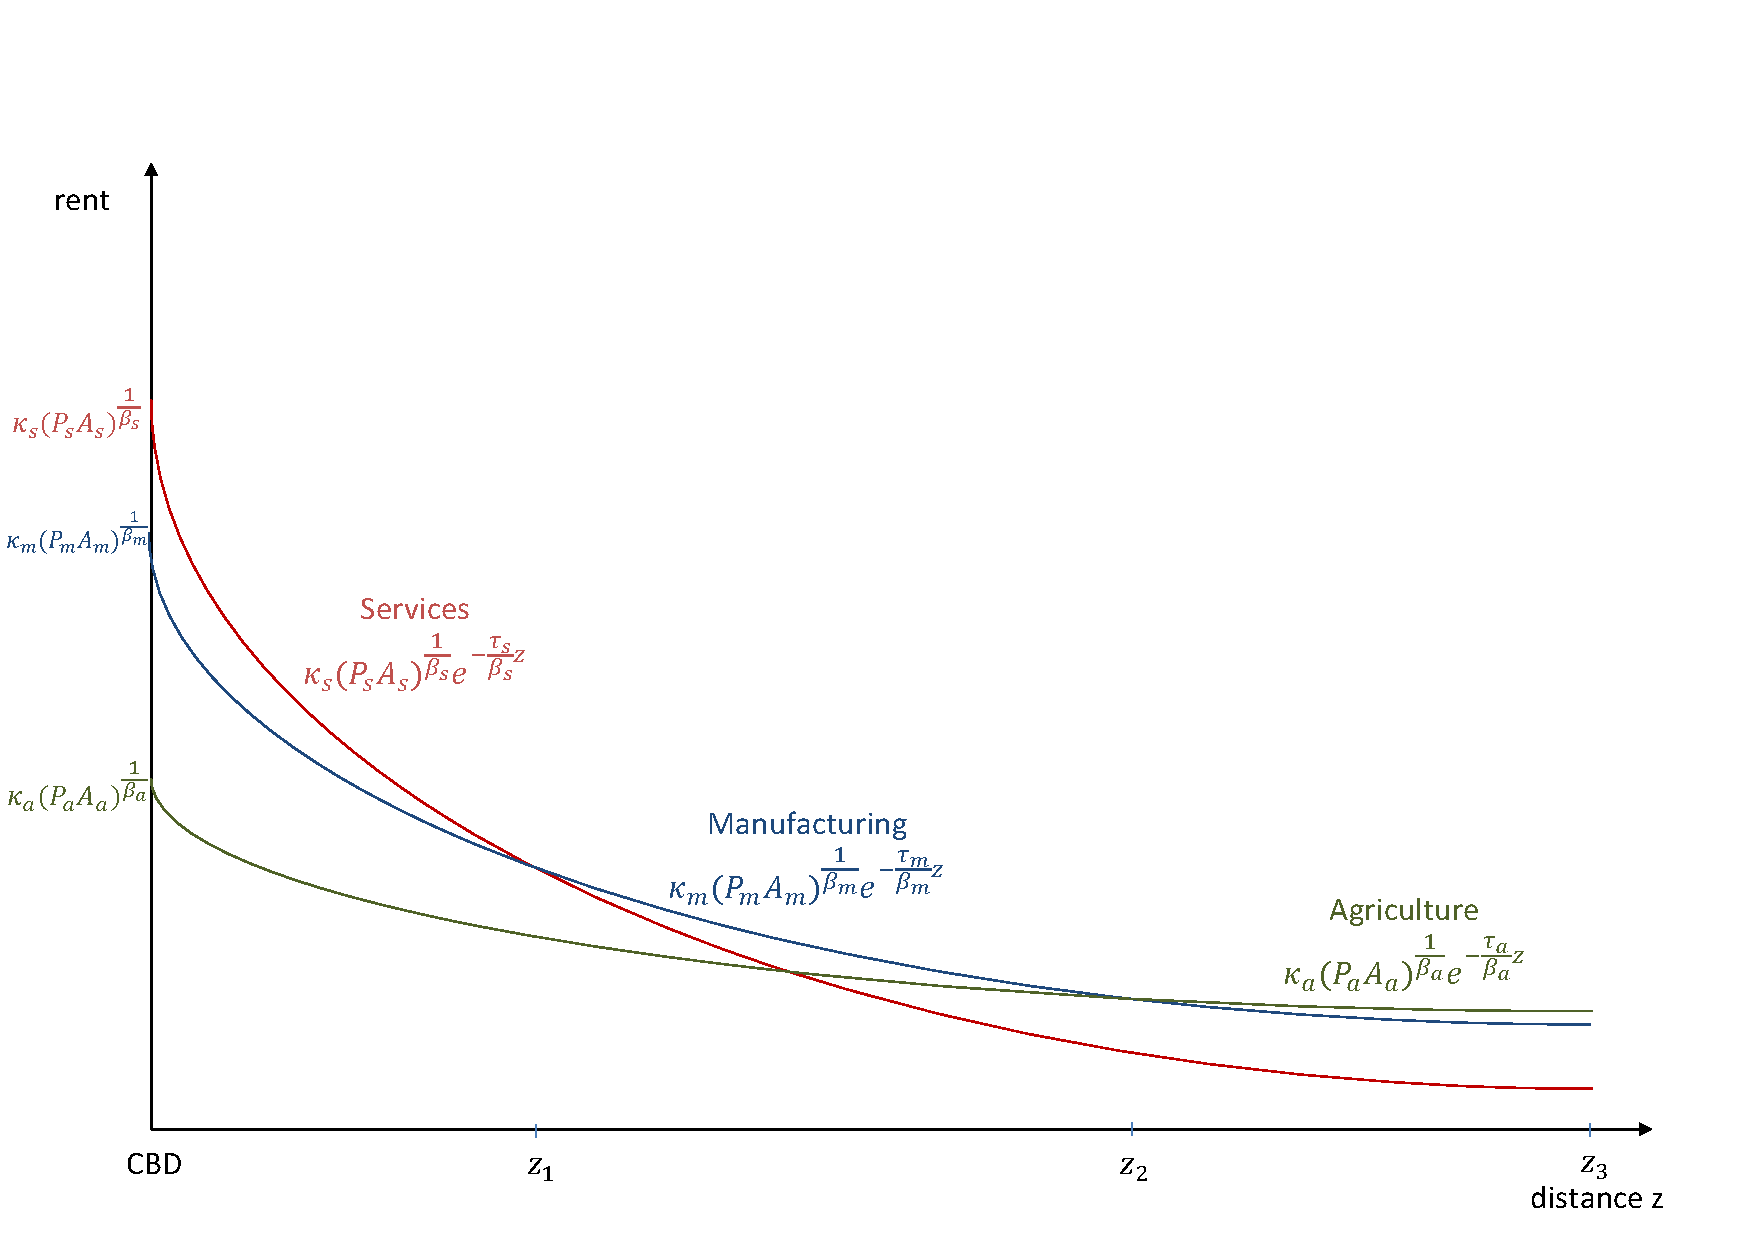
\includegraphics[scale=0.6]{figures/fig_spatial_equilibrium}
\end{center}

\noindent \footnotesize{The figure plots the structure of a spatial competitive equilibrium. It shows equilibrium sectoral bid rent curves as a function of distance from the city center. A sector is active over an area where it is willing to overbid alternative sectors. Crossings of the bid-rent curves determine the borders of the sectors. Services are active in $[0,z_1]$, manufacturing in $\left(z_1,z_2\right]$, and services in $\left(z_2,z_3\right]$.}
\end{figure}


\subsection{Spatial arbitrage}
Competitive land markets ensure that each location goes to the highest bidder. The slope of the bid-rent gradient in sector $i$ is $\tau_i/\beta_i$. Suppose that this is the highest for services, lower for manufacturing, and lowest for agriculture.

Let $z_i$ denote the outer edge of the land use of sector $i$. At such locations, both sector $i$ and sector $i+1$ have the same reservation rent:
\begin{align}\label{eq:BorderRents}
R(z_i) &=\beta_i(1-\beta_i)^{1/\beta_i-1} (P_iA_i)^{1/\beta_i} W^{1-1/\beta_i} e^{-\frac{\tau_i}{\beta_i} z_i}\\
R(z_i) &=\beta_{i+1}(1-\beta_{i+1})^{1/\beta_{i+1}-1} (P_{i+1}A_{i+1})^{1/\beta_{i+1}} W^{1-1/\beta_{i+1}} e^{-\frac{\tau_{i+1}}{\beta_{i+1}} z_i}
\end{align}
Substitute in the overall amount of value added, $Y_i = P_iQ_i$,
\[
R_i(z) = R_i e^{-\frac{\tau_i}{\beta_i}(z-\tilde z_i)}.
\]
\[
R_i = \frac{\beta_i Y_i}{L_i}
\]
\[
R_i(z) = \frac{\beta_i Y_i}{L_i} e^{-\frac{\tau_i}{\beta_i}(z-\tilde z_i)}.
\]
At the location $z_{i-1}$ where sectors $i$ and $i-1$ meet,
\[
\frac{\beta_{i-1} Y_{i-1}}{L_{i-1}}
  e^{-\frac{\tau_{i-1}}{\beta_{i-1}}(z_{i-1}-\tilde z_{i-1})} =
\frac{\beta_i Y_i}{L_i}
  e^{-\frac{\tau_i}{\beta_i}(z_{i-1} -\tilde z_i)}.
\]
To solve for the barriers, we use the fact that $Y_{i-1}/Y_i = \alpha_{i-1}/\alpha_i$,
\[
\frac{\alpha_{i-1}\beta_{i-1} }
{\alpha_i \beta_i}
=
\frac{\int_{z\in Z_{i-1}} \tilde L(z) dz}
{\int_{z\in Z_{i}} \tilde L(z) dz}
  e^{\frac{\tau_{i-1}}{\beta_{i-1}}(z_{i-1}-\tilde z_{i-1})-\frac{\tau_i}{\beta_i}(z_{i-1} -\tilde z_i)}.
\]



\subsection{Solving for the prices}

At the sector borders $z_i$, neighboring sectors have the same reservation rents. Having solved for these locations, equations \ref{eq:BorderRents} provide implicit equations for relative product prices $P_i$ for $i=s,m.$ The consumer budget constraint, given by equation \ref{eq:BudCons}, gives us the equation for the remaining product price $P_a$. This closes the model description.   


\subsection{Linear city}
A linear city is one with $\tilde L(z) = l$ everywhere. 
\[
\tilde z_i = z_{i-1} - \frac{\beta_i}{\tau_i}
\ln
\frac{1-e^{-\frac{\tau_i}{\beta_i} (z_{i} - z_{i-1}) }}
{\tau_i/\beta_i}.
\]

\[
e^{\frac{\tau_i}{\beta_i}(\tilde z_i - z_{i-1} )}
=
\frac
{\tau_i/\beta_i}
{1-e^{-\frac{\tau_i}{\beta_i} (z_{i} - z_{i-1}) }}
\]

\[
e^{\frac{\tau_{i-1}}{\beta_{i-1}}(z_{i-1}-\tilde z_{i-1})} =
e^{\frac{\tau_{i-1}}{\beta_{i-1}}(z_{i-1}-z_{i-2}+z_{i-2}-\tilde z_{i-1})} =
e^{\frac{\tau_{i-1}}{\beta_{i-1}}(z_{i-1}-z_{i-2})}
e^{-\frac{\tau_{i-1}}{\beta_{i-1}}(\tilde z_{i-1}-z_{i-2})} =
\]
\[
e^{\frac{\tau_{i-1}}{\beta_{i-1}}(z_{i-1}-z_{i-2})}
\frac
{1-e^{-\frac{\tau_{i-1}}{\beta_{i-1}} (z_{i-1} - z_{i-2}) }}
{\tau_{i-1}/\beta_{i-1}}
\]

In this case, spatial arbitrage dictates
\[
\frac{\alpha_{i-1}\beta_{i-1} }
{\alpha_i \beta_i}
=
\frac{z_{i-1}-z_{i-2}}
{z_i - z_{i-1}}
  e^{\frac{\tau_{i-1}}{\beta_{i-1}}(z_{i-1}-\tilde z_{i-1})-\frac{\tau_i}{\beta_i}(z_{i-1} -\tilde z_i)}.
\]
which becomes
\[
\frac{\alpha_{i-1}\beta_{i-1} }
{\alpha_i \beta_i}
=
e^{\frac{\tau_{i-1}}{\beta_{i-1}}(z_{i-1}-z_{i-2})}
\left(\frac{z_{i-1}-z_{i-2}}
{z_i - z_{i-1}}\right)^2
\frac
{\frac{\tau_i}{\beta_i}(z_{i} - z_{i-1})}
{1-e^{-\frac{\tau_i}{\beta_i} (z_{i} - z_{i-1}) }}
\frac
{1-e^{-\frac{\tau_{i-1}}{\beta_{i-1}} (z_{i-1} - z_{i-2}) }}
{\frac{\tau_{i-1}}{\beta_{i-1}} (z_{i-1} - z_{i-2})}
\]
Using the approximation $1-e^{-x}\approx x$, the last two ratios are approximately one, so that
\[
\frac{\alpha_{i-1}\beta_{i-1} }
{\alpha_i \beta_i}
\approx
e^{\frac{\tau_{i-1}}{\beta_{i-1}}(z_{i-1}-z_{i-2})}
\left(\frac{z_{i-1}-z_{i-2}}
{z_i - z_{i-1}}\right)^2.
\]
To understand the intuition for this spatial aribtrage condition, suppose we increase $z_{i-1}$. This has two effects. First, it increases the land available to produce good $i-1$. Second, it raises the rent gradient so that the equality between sectors $i$ and $i-1$ happens at the new location. Both effects increase the total rent paid to sector $i-1$ relative to that paid to sector $i$. (Hence the quadratic term.) This is inconstitent with equilibrium, where total rents paid to the two sector are determined by the Cobb--Douglas coefficients.

\subsection{Circular city}




\section{Development accounting}
\subsection{Aggregation across space}
Sectoral production, as we show in this section, is a function of a suitably chosen representative location. 

Sectoral output measured at the center is
\begin{equation*}
\tilde{Q}_i=\int_{z\in Z_i}e^{-\tau_i z}A_iL_i(z)^\beta_iN_i(z)^{1-\beta_i}dz,
\end{equation*}
where $Z_i$ is the set of locations where sector $i$ is active in equilibrium. 

Let the representative location
\begin{equation}
\label{eq:ReprLoc}
\tilde z_i = -
\frac{\beta_i}{\tau_i}
\ln\int_{z\in Z_i} \frac{L_i(z)}{L_i}e^{-\frac{\tau_i}{\beta_i} z}dz
\end{equation}
denote the average distance of sector $i$ to the center, where $L_i=\int_{z\in Z_i} L_i(z)dz$ is the total amount of land devoted to sector $i$. This definition ensures that the trade cost going to location $\tilde z_i$ equals the land-weighted average trade cost across all sectoral locations,
\[
e^{-\frac{\tau_i}{\beta_i} \tilde z_i} = \int_{z\in Z_i} \frac{L_i(z)}{L_i}e^{-\frac{\tau_i}{\beta_i} z}dz.
\]
As we will see below, $\tilde z_i$ is a sufficient statistic about sector location for aggregation purposes. %(XX THIS IS A TRICK OF THE MELITZ MODEL)

\begin{proposition}
Aggregate sectoral production function is of the form: 
\begin{equation}
\tilde Q_i =
A_iL_i^{\beta_i}N_i^{1-\beta_i}
 e^{-\tau_i\tilde z_i}.
\end{equation}
It depends on trade costs from the representative location ($\tilde{z}_i$) defined by equation \ref{eq:ReprLoc} and is a Cobb-Douglas aggregate of sectoral land ($L_i=\int_{Z_i}L_i(z)dz$) and labor ($N_i=\int_{Z_i}N_i(z)dz$) use.
\end{proposition}

To show that it is the case, let us express value added (measured at the center) at a location $z$ per unit of land:
\[
\frac{e^{-\tau_i z} Q_i(z)}{L_i(z)} = e^{-\tau_i z} A_i(z)\left(\frac{N_i(z)}{L_i(z)}\right)^{1-\beta_i} = (1-\beta_i)^{1/\beta_i-1}
A_i^{1/\beta_i}\left(\frac{W}{P_i}\right)^{1-1/\beta_i}
 e^{-\frac{\tau_i}{\beta_i} z},
\]
where we used equation \ref{eq:EmpDens} on employment density. From this, total supply of sector $i$ becomes 
\begin{equation}
\label{eq:OutputInterm}
\tilde{Q_i} = \int_{z\in Z_i}\frac{e^{-\tau_i z} Q_i(z)}{L_i(z)}L_i(z)dz=(1-\beta_i)^{1/\beta_i-1}
(A_i)^{1/\beta_i}\left(\frac{W}{P_i}\right)^{1-1/\beta_i} L_i e^{-\frac{\tau_i}{\beta_i} \tilde z_i}.
\end{equation} 
by the definition of the representative location of the sector in equation \ref{eq:ReprLoc}.

Overall employment in the sector,
\[
N_i = \int_{z\in Z_i}\frac{N_i(z)}{L_i(z)}L_i(z)dz= (1-\beta_i)^{1/\beta_i}
\left(\frac{P_iA_i}{W}\right)^{1/\beta_i} L_i e^{-\frac{\tau_i}{\beta_i} \tilde z_i},
\]
so that we can express $W/P_i$ as
%\[
%\left(\frac{W}{P_i}\right)^{1/\beta_i} = (1-\beta_i)^{1/\beta_i}
%N_i^{-1}A_i^{1/\beta_i}
%L_i e^{-\frac{\tau_i}{\beta_i} \tilde z_i}
%\]
\[
\frac{W}{P_i} = (1-\beta_i)
N_i^{-\beta_i}A_i L_i^{\beta_i}
 e^{-\tau_i\tilde z_i}
\]
%\[
%\left(\frac{W}{P_i}\right)^{1-1/\beta_i} = (1-\beta_i)^{1-1/\beta_i}
%A_i^{1-1/\beta_i}N_i^{1-\beta_i}L_i^{\beta_i-1}
%e^{\frac{1-\beta_i}{\beta_i}\tau_i \tilde z_i}
%\]
Substituting this result to equation \ref{eq:OutputInterm}, we obtain the aggregate production function. 

\subsection{Productivity measurement}
Productivity measurements disregarding land and location lead to biased results, which we analyse below using our model. We first show the bias for labor productivity, which ignores land altogether, then for total-factor productivity, which accounts for land, but ignores its location.

%Suppose physical output is measured as revenue at producer prices deflated by a common price index. We take the price index to be the consumer price (XX CHECK IF IT MATTERS).
%\[
%\tilde Q_i(z) = \frac{e^{-\tau_i z}P_iQ_i(Z)}{P_i}
%\]
%We can write an aggregate output as
%\[
%\tilde Q_i =
%(1-\beta_i)^{1/\beta_i-1}
%A_i^{1/\beta_i}\left(\frac{W}{P_i}\right)^{1-1/\beta_i}
%L_i e^{-\frac{\tau_i}{\beta_i} \tilde z_i}
%\]
%which takes us to the aggregate production function
%\[
%\tilde Q_i =
%A_iL_i^{\beta_i}N_i^{1-\beta_i}
% e^{-\tau_i\tilde z_i}.
%\]
%Aggregate output is a Cobb--Douglas function of land and labor, adjusted with trade costs. The factor is smaller for sectors with large trade costs ($\tau_i$) and sectors farther away from the city (larger $\tilde z_i$). 

Sectoral output per worker is
\[
\frac{\tilde Q_i}{N_i} = \frac1{1-\beta_i}
\frac{W}{P_i}.
\]
We can substitute out product prices in this formula and express them as a function of input costs. To do this, define average sectoral rents as
\begin{equation}
R_i =\int_{z\in Z_i}\frac{L_i(z)}{L_i}R(z)dz = \beta_i(1-\beta_i)^{1/\beta_i-1} \left(P_iA_i\right)^{1/\beta_i} W^{1-1/\beta_i} e^{-\frac{\tau_i}{\beta_i} \tilde{z}_i}
\end{equation}
Note that $R_i$ also equals to the rent prevailing at location $\tilde z_i$. From this, we get that 
%\[
%\frac{R_i}{W} =\beta_i(1-\beta_i)^{1/\beta_i-1} \left(\frac{P_iA_i}{W}\right)^{1/\beta_i} e^{-\frac{\tau_i}{\beta_i} \tilde z_i},
%\]
%where $R_i$ is the rent prevailing at location $\tilde z_i$ (which is also equal to the average rent paid by the sector, as proven below)
%\[
%R(\tilde z_i) =
%R(z_{i-1})e^{-\frac{\tau_i}{\beta_i}(\tilde z_i-z_{i-1})}
%\]

%\[
%\left(\frac{W}{P_i}\right)^{1/\beta_i}  =\beta_i(1-\beta_i)^{1/\beta_i-1}
%A_i^{1/\beta_i}
%\frac{W}{R_i}
% e^{-\frac{\tau_i}{\beta_i} \tilde z_i}
%\]
\[
\frac{W}{P_i}  =\beta_i^{\beta_i}(1-\beta_i)^{1-\beta_i}
A_i
\left(\frac{W}{R_i}\right)^{\beta_i}
 e^{-\tau_i \tilde z_i}
\]
so that output per worker can be written as
\begin{equation}
\frac{\tilde Q_i}{N_i} = \beta_i^{\beta_i}(1-\beta_i)^{-\beta_i}
A_i
\left(\frac{W}{R_i}\right)^{\beta_i}e^{-\tau_i \tilde z_i}.
\end{equation}

Log output per worker is
\[
\tilde q_i - n_i =
\beta_i\ln\beta_i+(1-\beta_i)\ln(1-\beta_i)
+a_i +\beta_i (w
-r_i)
- \tau_{i}\tilde z_{i}
\]
Conditional on true productivity $a_i$, measured productivity (ignoring land) is lower in cities where rents are higher. The magnitude of this bias depends on the (direct and indirect) land share of the sector, $\beta_i$. Measured productivity is also lower whenever the sector locates far from the center ($\tilde z_i$ is high). %Interestingly, this bias does not depend on the land share. The intuition is that XX
The former bias will be bigger for rich countries, as rents tend to be more sensitive to per capita income than wages are. The latter bias will be bigger for rich and urbanized countries, where each urban sector takes up more space. Simply put, services will look unproductive in New York City relative to Budapest, because NYC is larger.

The bias in measured total factor productivity (if location is ignored) depends on sectoral trade costs ($-\tau_i\tilde z_i$), as 
\begin{equation}
\frac{\tilde Q_i}{L_i^{\beta_i}N_i^{1-\beta_i}} = A_i e^{-\tau_i \tilde z_i}.
\end{equation}
The bias is higher in non-tradable sectors, and in large countries and cities. 

We can calculate an alternative measure of TFP, valuing the stock of land at market prices (or, rather, market rents),
\[
\tilde L_i = R_iL_i = R_i(0)e^{-\frac{\tau_i}{\beta_i}\tilde z_i}L_i.
\]
This ensures that
\[
\frac{\tilde Q_i}{\tilde L_i^{\beta_i}N_i^{1-\beta_i}} = 
\frac{A_i}{R_i(0)^{\beta_i}}
= \frac{W^{1-\beta_i}}{P_i}\beta_i^{-\beta_i}(1-\beta_i)^{-(1-\beta_i)}
\]


\subsection{Development accounting} 
Location-corrected productivity can be expressed from measured TFP as
\[
a_i =  \tilde a_i+ \tau_{i}z_{i},
\]
where $\tilde a_i$ is log measured total-factor productivity productivity. This is our main equation for sector-level development accounting.

We are interested in how location-corrected sectoral productivities are correlated with per capita income.
\[
\frac{d a_i}{dy_i} = \frac{d \tilde a_i}{dy_i}+ \tau_{i}\frac{d \tilde z_i}{dy_i}.
\]
For this, we need a solution to sector-specific location variables as a function of observables.  

\subsection{Sectoral allocation of land}
We want to express the sectoral allocation of land as a function of GDP shares of sectors,  which, in contrast to land shares, are observable in NIPA.\footnote{Value productivity $P_iA_i$ and trade costs $e^{-\tau_i \tilde z_i}$ are completely isomorphic in the sense that they only appear together in our aggregate equations. That is, we cannot calibrate $\tau$ and $\tilde z$ from aggregate data alone. We will calibrate these from ZIP-code-level data in the U.S., and use data on $P_iA_i$ for other countries.} Land demand per dollar of value added,
\[
\frac{L_i}{Y_i} =
\frac{\beta_i}{R_i}.
\]
Using the formula for the rent gradient, 
\[
\frac{L_i}{Y_i} =
(1-\beta_i)^{1-1/\beta_i} (P_iA_i)^{-1/\beta_i}W^{1/\beta_i-1} e^{\frac{\tau_i}{\beta_i} \tilde z_i}.
\]
We rewrite this in terms of land and GDP shares,
\[
\frac{L_i}{L} = \frac{Y_i}{Y}\frac{Y}{WL}
(1-\beta_i)^{1-1/\beta_i}\left(\frac{W}{P_iA_i e^{-\tau_i\tilde z_i}}\right)^{1/\beta_i}.
\]
Note that the last term is unit labor cost, and, given that \emph{measured} TFP is $A_i e^{-\tau_i\tilde z_i}$, all its components are, in principle, measurable.

Let superscript $j$ denote country $j$ (we have omitted country indexes so far).
\begin{equation}
\label{eq:LandShare}
\frac{L_i^j}{L^j} = \frac{Y_i^j}{Y^j}\frac{Y^j}{W^jL^j}
(1-\beta_i)^{1-1/\beta_i}\left(ULC_i^j\right)^{1/\beta_i} ,
\end{equation}
and we have denoted by
\[
ULC_i^j
=
\frac{W}{P_iA_i e^{-\tau_i\tilde z_i}}
\]
the measured unit labor cost in country $j$ in sector $i$.

The land share of a sector is increasing in its land intensity $\beta_i$ (assumed common across countries), GDP share ${Y_i^j}/{Y^j}$ (can differ across countries for a variety of reasons), and its unit labor cost. Intuitively, sectors with high unit labor cost use more land to economize on labor.

To measure the unit labor cost, we need to choose the units of each sector. To do this, we look at the actual land usage of sectors in the U.S. and choose units in such a way that U.S. unit labor costs are 1 for each sector,
\begin{equation}
\label{eq:US_ULC}
ULC_i^{USA} =1=(1-\beta_i)^{\beta_i-1} \left(\frac{L_i^{USA}}{Y_i^{USA}}\right)^{\beta_i}(W^{USA})^{\beta_i}
\end{equation}
Having the proper units of output (and ULC), we can simply calculate the land demand in each country for a set of value added shares and measured ULCs.


\section{Multiple Cities}
So far we have discussed the equilibrium of a given city, with a fixed supply of land and labor. In this section, we introduce a system of multiple cities within a country. We first discuss the case when the number of cities is fixed, but their area and population are endogenous. We then turn to endogenizing the number of cities with development.

To endogenize the boundaries of cities, we have to take a stand on what happens ``in between'' cities. Following the tradition of the urban literature, we assume that agricultural goods are freely tradable, $\tau_3=0$. As we show below, this assumption ensures that agriculture fills up all the space between cities. The urban fringe is then $z_2$.

When agriculture is freely tradable, its rent gradient is completely flat. Agricultural producers are indifferent as to where they locate.

\subsection{Fixed number of cities}
Let the country have $k=1,2,...,K$ cities. Each city has a CBD in an exogenously fixed location. We assume the country is large enough that cities boundaries never overlap. 

Cities also differ in labor productivity. In particular, city $k$ is characterized by a labor productivity shifter $\Omega_k$, so that the effective supply of labor is $\Omega_kN_k$, where $N_k$ is the population of the city. 

We need some heterogeneity across cities to capture the empirical fact that cities differ in size. Desmet and Rossi-Hansberg (XX) build a model where cities differ in productivity, amenities and the efficiency of public services. We focus on productivity to capture the most salient differences across cities. We also note that better amenities are similar to higher labor productivity in that they reduce the unit labor cost in the city: A likeable city offers low wages, making it cheap to produce there.

An \emph{equilibrium system of cities} consists of a list of city populations $\{N_k\}$, city boundaries $\{z_{k2}\}$ XX
such that
(i) each city is in a \emph{single-city equilibrium} given its boundary $z_{k2}$ and population $N_k$, (ii) land rents at the urban fringe are equal to agricultural rents, (iii) workers earn the same real wage in each city, (iv) the sum of city population and rural population equals country population.

\subsubsection{Equilibrium allocation of workers}
Free worker mobility equates real wages across cities. In fact, as the point of consumption is independent from the point of employment (we need this assumption so that agricultural workers can also consume urban goods), the law of one price will prevail for all goods across all cities. This will equate the nominal wage, as well. The only thing that differs across productive and unproductive cities is the urban rent.\footnote{To be consistent with the free trade of consumption goods, we can reinterpret the CBD as providing a necessary service in the \emph{production}, but not the consumption of goods, e.g., packaging.}

\subsubsection{Urban sectors}
The supply of urban sectors in each city is characterized by the single-city equilibrium, adjusted for city-level labor productivity shifter,
\[
Q_m = A_m\Omega_k^{1-\beta_m}e^{-\tau_m\tilde z_{km}} 
L_{km}^{\beta_m}
N_{km}^{1-\beta_m}.
\]
The rent gradient is modified with the city-specific labor productivity,
\[
R_{ki}(z) =\beta_i(1-\beta_i)^{1/\beta_i-1} (P_iA_i)^{1/\beta_i} (W/\Omega_k)^{1-1/\beta_i} e^{-\frac{\tau_i}{\beta_i} z}.
\]
The boundary between the two urban sectors is determined by the relative price,
Because the law of one price holds for urban sectors, 
\subsubsection{Arbitrage at the urban fringe}
Urban rent at the fringe $z_{km}$ equals agricultural rent,
\[
R_{km}(z_{km}) = R_a = R_{km}(0)e^{-\frac{\tau_m}{\beta_m}z_{km}}.
\]
Given that product prices are the same in each city, we can write this arbitrage condition as
\[
\Omega_k^{1/\beta_m-1}e^{-\frac{\tau_m}{\beta_m}z_{km}}
=\frac1{\beta_m}
(1-\beta_m)^{1-1/\beta_m}
\frac{R_a}{W}
\left(
\frac{P_mA_m}{W}
\right)^{-1/\beta_m}
\]
Importantly, none of the terms on the RHS depend on $k$. We can hence derive the relative boundary of any two cities as
\[
(1-\beta_m)(\omega_{k} - \omega_{k'}) = 
\tau_m(z_{km} - z_{k'm}).
\]
More productive cities are larger.

\subsubsection{Rural land}
We still need to determine the overall quantity of rural vs urban land and employment. The ratio of urban to rural labor,
\[
\frac{N_m+N_s}{N_a} =
\frac{WN_m/Y+WN_s/Y}{WN_a/Y} = 
\frac{\alpha_m(1-\beta_m)+\alpha_s(1-\beta_s)}{\alpha_a(1-\beta_a)}
\]
is constant. The same ratio for land rents,
\[
\frac{\sum_k \tilde R_{ks}L_{ks}+\tilde R_{km}L_{km}}
{R_aL_a} = 
\frac{\alpha_m\beta_m+\alpha_s\beta_s}{\alpha_a\beta_a}.
\]
This suggests the following algorithmic construction of the quilibrium
\begin{enumerate}
\item Guess $L_a$. This also fixes urban land $L-L_a$.
\item Given the relative city sizes and the total urban land, calculate the urban fring for each city $\{z_{km}\}$.
\item Solve for the single-city equilibrium to determine $\{z_{ks}\}$. (XX CHALLENGE: we do not have market clearing by city, they may become specialized in either urban good)
\item Given $\{(z_{ks}, z_{km})\}$, solve for the rent gradient in each city and calculate total urban rents.
\item If urban rents are too high relative to rural rents, reduce $L_a$ and go back to step (1). 
\end{enumerate}
\subsection{Endogenous cities}
Urbanization clearly varies with development (XX REF). We introduce an extension of the model that is consistent with this empirical patterns. The extended model leads to additional predcitions that can be tested against the data.

A country is characterized by a triplet of productivities in the three sectors, $(A_s, A_m, A_a)$, total population $N$, and total land area $L$. The country can build cities at a fixed cost $f$ each. Each city has a random labor productivity $\Omega_k$, drawn independently from the common distribution $\Phi(\Omega)$.

An \emph{endgenous-city equilibrium} is XX.

\section{Data and calibration}
Now we calibrate the model to show that correcting for land and location in sectoral productivity measures has the potential to change previous conclusions of multi-sector development accounting.
We allow for sector-specific differences in productivity ($A_i$), which are the key object of interest in multi-sector development accounting. The urban fringe ($z_3$) may also vary with country area and its degree of urbanization and we calibrate it below. Demand parameters ($\alpha_i$) are allowed to vary to allow different countries to have different expenditure shares in agriculture, manufacturing and services. %XX TALK MORE ABOUT STRUCTURAL CHG
Each country has the same land share within sectors $\beta_i$ and the same shipping cost $\tau_i$.
%\subsection{Variation across countries}
%Countries differ in Hicks-neutral productivities $A_i$, their urban fringe $z_3$ and their demand parameters $\alpha_i$.

\subsection{Calibration}
First we calibrate land shares and shipping costs using US data. Then we turn to the calibration of parameters influencing cross-country variations.

\subsubsection{Land shares}
We calibrate sectoral land shares ($\beta_i$) using US data. Our aim is to capture the share of immobile factors in production. These come from two sources: $(i)$ the direct use of land in production and $(ii)$ the land-rent paid by workers. We calibrate the direct use of land in sectoral production using US factor income share estimates of \citeN{Valentinyi08}. The first two columns of table \ref{tab:Sector_Shares} show their estimates for land and labor shares across sectors.

The indirect use of land is the land used by workers. We calibrate land-rent share in labor as a product of the US aggregate rent-share in consumption expenditure reported by the BLS ($30\%$) and the average land-share of US house prices between 1984-1998 estimated by \citeN{Davis08} (36\%). We find it to be 10.8\%. We multiply this by the labor shares to get the indirect land shares listed in column 3 of table $\ref{tab:Sector_Shares}$. Our calibrated overall land shares ($\beta_i$) are the sum of the direct and indirect land shares, and they are shown in column 4.

The calibrated values show that land is a non-negligible factor in production in each sectors. As expected, its role is the largest in agriculture (23\%), but the land share in manufacturing and services are both double-digit (10\%-13\%), mainly because of the indirect land use of their workers.


\begin{table}[h!]
\label{tab:Sector_Shares}
\caption{Calibrated factor shares}
\begin{center}
\begin{tabular}{l|ccc|c}
\toprule
Factor shares & Direct land & Labor & Indirect land & Overall land share $\beta_i$ \\
\midrule
Agriculture & 0.18 & 0.46  & 0.05 & 0.23 \\
Manufacturing& 0.03 & 0.67 & 0.07 & 0.10  \\
Services    &  0.06 & 0.66 & 0.07 & 0.13 \\
\bottomrule
\end{tabular}
\end{center}

\noindent \footnotesize{Land and Labor shares are estimates of \citeN{Valentinyi08}. Land share in labor is the product of rent-share in US consumption expenditures, the average land-share of US house prices between 1984-1998 estimated by \citeN{Davis08} and the labor shares. Our land share estimates are the sum of direct land share and the indirect land share in labor.}
\end{table}

\subsubsection{Shipping costs}

We use the 2010 ZIP Business Patters of the U.S. Census to determine the location of sectors in the United States. We use this to calibrate transportation costs and distances of the sectors from the center.

The ZIP Business Patterns contains the number of establishments in employment size categories in each ZIP code for each 6-digit NAICS code. We merge NAICS codes into agriculture, manufacturing and services as follows. Agriculture is sector 11 of NAICS. We merge mining (21), utilities (22), and construction (23) together with manufacturing industries (31-33). As services, we categorize the rest, including public administration. We estimate employment by using the midpoints of the size categories.

To map the model into the data, we need to specify how far each ZIP code is from the city center. We take Urbanized Areas (UAs) as independent monocentric cities, and we assign the central point to the business or administrative center of the first-mentioned city in the UA, as given by Yahoo Maps. For example, the center of ``New York–Newark, NY-NJ-CT Urbanized Area'' is the corner of Broadway and Chamber St in downtown Manhattan, whereas the center of ``Boston, MA–NH-RI Urbanized Area'' is 1 Boston Pl. We calculate the distance of each ZIP code to business center of the nearest UA.

According to equation \ref{eq:EmpDens}, the employment density of sector $i$ in location $z$ is proportional to the rent-wage ratio. When industry $i$ demands positive land in the neighborhood of $z$, then the rent is proportional to $e^{-\tau_i/\beta_i z}$. We can use this observation to estimate $\tau_i$:
\[
\frac{d\ln n_i(z)/l_i(z)}{dz} =\frac{d\ln r_i(z)}{dz} = -\frac{\tau_i}{\beta_i}.
\]

To get a sense where each sectors is active, we calculate location quotients by distance to the city center. For each sector, they measure the employment share at a certain distance relative to the average employment share of the same sector. A value higher than 1 implies that the sector is overrepresented in the particular distance from the center.

\dofigure{sector_location_quotients}{Sector location quotients}{Source: ZIP Business Patterns. Plots the sectoral employment shares at a particular distance (in a 3kms wide ring) from the city center, relative to the average sectoral employment share. The figure shows that sectors sort as in the model: services are overrepresented closer the the city center, while manufacturing and agriculture are located mostly farther away, agriculture showing a particularly steep gradient.}

Figure \ref{fig:sector_location_quotients} shows that sectors sort as in the model: services are overrepresented closer to the city center, while manufacturing and agriculture are both underrepresented there. Agriculture shows a particularly steep gradient, with high relative employment farther away from the city center. In the calculation of sectoral employment gradients below, we restrict attention to the areas where the sectors are overrepresented. We assume that services are active up to 30 kms from the center, manufacturing is active between 10 and 60 kms and agriculture farther than 60 kms.

Let $n_{izc}$ be the employment of industry $i$ in ZIP code $z$, belonging to city (MSA) $c$.  Assuming that establishments in a given sector consume the same amount of land,\footnote{We believe this approximation is likely to bias our estimates of the rent gradient downward. Rural establishments probably occupy more space that urban establishments even in the same narrow industry, so establishment sizes do not go down as fast with distance as employment density does. } we denote by $l_{izc}$ the number of establishments of sector $i$ in ZIP code $z$. We can then regress establishment size (workers per establishment) in each sector in each ZIP code on fixed effects, and the distance of the ZIP code to the city center,
\begin{equation}\label{eq:estimable:gradient}
\frac{n_{izc}}{l_{izc}} = e^{\mu_c+\nu_i-\gamma_i d(z,c)}.
\end{equation}
The city fixed effect captures variation in rents and wages in the MSA, the sector fixed effect captures variation in land and labor intensity and establishment size across sectors. %XX WE MAY NEED CITY*SECTOR FEs
The key parameter of interest is $\gamma_i$, which captures how fast employment declines with distance to the center by sector.

\subsubsection{Imputing employment density at the ZIP-code level}
From the ZBP, we have the approximate employment of the sector (reconstructed from establishment-size bins), and the total area of the ZIP code, but area is not broken down by sector. If a ZIP code is exclusively used by one of the three sector, this is not a problem. Otherwise, we impute the area used by sector $i$ as follows.

The mode predicts the area per worker in sector $i$ in ZIP-code $z$ to be
\[
\frac{L_i(z)}{N_i(z)} = \frac{1-\beta_i}{\beta_i}\frac{W}{R(z)}.
\]
Because all sectors face the same wages and rents in the same ZIP code, we can distribute land in proportion to
\[
\frac{1-\beta_i}{\beta_i}N_i(z).
\]
In urban ZIP codes, there is also a substantial amount of residential land. We know that households spend $0.3\times 0.36$ fraction of their income on residential land rent. Assuming that residents' only income are wages,
\[
\frac{R(z)H(z)}{WP(z)} = 0.3\times 0.36,
\]
where $P(z)$ is the number of people living in ZIP code $z$. Hence total residential area is
\[
H(z) = 0.3\cdot0.36 P(z) \frac{W}{R(z)}.
\]
We then allocate residential land in proportion to $0.3\cdot0.36 P(z)$.

We estimate \eqref{eq:estimable:gradient} by a Poisson regression which ensures that the equation holds in expectation, and permits estimation even when $n_{izc}=0$, which is often the case. The estimates of $\gamma_i$ and the implied sectoral transport cost intensities $\tau_i$ in the three sectors are below.

% Table generated by Excel2LaTeX from sheet 'tau'
\begin{table}[h!]
  \begin{center}
  \caption{Estimated rent and price gradients}
    \begin{tabular}{rccc}
    \toprule
    \textbf{} & \textbf{} & \multicolumn{2}{c}{\textbf{Gradient (per km)}}\\
    \midrule
    \textbf{} & \textbf{Land share $\beta_i$ } & \textbf{Rents $\gamma_i$} & \textbf{Prices $\tau_i$} \\
    Services & 13\%  & 13.15\% & 1.71\% \\
    Manufacturing & 10\%  & 5.15\% & 0.52\% \\
    Agriculture & 23\%  & 3.54\% & 0.81\% \\
    \bottomrule
    \end{tabular}%

  \end{center}
  \label{tab:EmpGrad}%

  \noindent \footnotesize{Sectoral rent gradients $\gamma_i$ are estimated using US employment-density observation across ZIP codes in MSAs. Price gradients reflect transport costs ($\tau_i$) and are estimated by multiplying rent gradients with sectoral land shares ($\beta_i$). }
\end{table}%

The three columns report the calibrated land shares, and the estimates for rent and price gradients, respectively, for each sector. The estimated coefficients can be interpreted as follows. We find that the rents paid by services become 13.15\% cheaper with every kilometer from the city center over the 0-30kms range, where services are active. Though a 13\% reduction is substantial, it does not seem unrealistic with a whole 1 kilometer distance. In line with our intuition, rent gradients of manufacturing and agriculture (measured further away from the city center) both imply slower rent declines. We infer price gradients reflecting the transportation cost intensities ($\tau_i$) from the measured rent gradients $\gamma_i=\tau_i/\beta_i$ and the sectoral land shares. The last column of table \ref{tab:EmpGrad} shows that we find transportation costs of services significantly higher (1.71\%) than those of manufacturing and agriculture (0.52\%, 0.81\%). We hold these estimated technology parameters constant across countries. %The employment density gradient of agriculture is inverted, reflecting the fact that most agricultural activity is carried out away from the cities.

\subsubsection{Country parameters}
We allow three parameters to vary across countries: the sector share of GDP ($\alpha_i$), the sectoral unit labor costs ($ULC_i$) and the city sizes $(z_3)$.

To capture the international variation in sectoral demand ($\alpha_i$), we use sectoral value added shares reported by the World Bank's World Development Indicator database.

The sectoral unit labor costs come from the EUKLEMS database (\citeN{OMahony09}), which contains internationally comparable sector-level labor compensation measures per hour and labor productivities.\footnote{Using multi-factor productivities would reduce our sample size from the already tight 14 to 11.}

The diverse \emph{size} of the representative cities introduces international variation in transport costs. To control for this, we take the internationally comparable ``arable land'' measure from the World Bank's World Development Indicator database\footnote{Some urban land measure would be preferable, but the available measures are based on national definitions, so can not be directly compared internationally.} and divide it by the number of cities with above 50.000 inhabitants.\footnote{The dataset is compiled by Stefan Helders (www.world-gazetteer.com) and uses mostly official sources.} This gives us a measure of the available land in the representative city. As we assume circular cities in our model, this area measure ($L$) readily translates into distance by $L=z_3^2\pi$, where $z_3$ the distance of the urban fringe from the city center $z_3$. Combining these measures with country-level estimates of sectoral land shares, as we show below, we obtain estimates for sectoral transport costs.

\subsubsection{Sector locations}

International variation in the distances of sectors from the city center influence transport costs. Our sector location measure ($z_i^j$) is a product of the urban fringe and sectoral land shares:\footnote{In the current version, we are calculating the maximum distance ($z_i^j$), instead of the average distance ($\tilde{z}_i^j$) suggested by the model. In this way, we are going to get a measure for the maximum bias to productivity estimates by disregarding location. It shows the potential of location correction. In the future versions, we are planning to use the model-based estimates of average sectoral distances.}
\begin{equation*}
z_i^j=z_3^j\sqrt{\frac{L_i^j}{L^j}}
\end{equation*}
For the US, we calculate sectoral land shares directly using the ZIP Business Patterns of the US Census. For each ZIP area, we calculate sectoral land demand as a share of commercial land, using the published employment data. %XX HOW?

Sectoral land share estimates for other countries are obtained using equation \ref{eq:LandShare}. The equation considers international variation in both sector demand and unit labor costs. As unit labor costs in EUKLEMS are expressed relative to the US, we choose the units of each sectors such that US unit labor costs are 1 (see equation \ref{eq:US_ULC}). Table \ref{tab:spatial_eg} compares estimates for three countries: a large developed country (USA), a small developed country (Belgium), and a small middle-income country (Hungary). Service sector constitute a large share of output in each countries, its share is somewhat smaller in the less developed Hungary. Agriculture, in contrast, generates only 1\% of the GDP in developed countries, but is somewhat more important in Hungary. Intuitively, sectors are closer to the city center of the representative cities in the smaller Belgium and Hungary than in the US.

% Table generated by Excel2LaTeX from sheet 'regions'
\begin{table}[h!]
  \centering
  \caption{Calibrated spatial structures}
    \begin{tabular}{rcccccc}
    \toprule
    \textbf{} & \multicolumn{3}{c}{\textbf{Share in GDP}} & \multicolumn{3}{c}{\textbf{Distance to center (km)}} \\
    \midrule
    \textbf{} & \textbf{USA} & \textbf{BEL} & \textbf{HUN} & \textbf{USA} & \textbf{BEL} & \textbf{HUN} \\
    Services & 77\%  & 75\%  & 66\%  & 36    & 15    & 8 \\
    Manufacturing & 22\%  & 24\%  & 30\%  & 39    & 16    & 14 \\
    Agriculture & 1\%   & 1\%   & 4\%   & 63    & 21    & 37 \\
    \bottomrule
    \end{tabular}%
  \label{tab:spatial_eg}%
\end{table}%

\subsection{Development accounting}

Which sector's productivity varies more with development? Our estimates for shipping costs and sector locations allow us to create location-corrected sectoral productivity measures $A_i$ from measured productivities $A_ie^{-\tau_iz_i}$. We are interested in their correlation with aggregate productivity. Our measured productivities come from 14 countries in the EUKLEMS database, and we compare them to GDP per capita from the 2007 World Development Indicators. Table \ref{tab:dev_acc} presents the estimated elasticities.

% Table generated by Excel2LaTeX from sheet 'devacct'
\begin{table}[h!]
  \centering
  \caption{Elasticity of productivity with respect to GDP per capita}
    \begin{tabular}{rcc}
    \toprule
    \textbf{} & \textbf{Measured} & \textbf{Location-corrected} \\
    \midrule
    Services & 0.628 & 0.855 \\
    Manufacturing & 0.867 & 0.926 \\
    Agriculture & 1.634 & 1.806 \\
    \bottomrule
    \end{tabular}%
  \label{tab:dev_acc}%
\end{table}%

We find that land and location of sectors do influence sectoral productivity measurements. Our preliminary results support previous conclusions that productivity differences in agriculture vary most with development. Correcting for the location-bias, this variation with development is, if anything, even higher. Using measured productivity, services productivity varies less with development than manufacturing productivity, in line with previous result. Correcting for the location-bias, however, changes this picture. It suggests that the cross-country differences in services productivity relative to manufacturing might be overestimated, because in our sample of high and middle-income countries location-corrected services productivity vary \emph{similarly} with development.

%\subsection{Sector locations}
%The plan for calibration is as follows.
%\begin{enumerate}
%    \item Normalize U.S. wages to one.
%    \item Measure the share of land in each sector in the U.S.
%    \item Use equation XX to obtain $P_iA_i$ for the U.S.
%    \item Given the measures of $P_iA_i$ and $W$ relative to the U.S. in EUKLEMS, we derive land demand in other countries using equation XX.
%\end{enumerate}
%
%\subsection{Trade costs}
%\begin{enumerate}
%    \item Guess $\tau_i$.
%    \item Given this guess, calculate the land-weighted distance of each sector in the U.S., $\tilde z_i$.
%    \item Calculate the same thing in the model.
%\end{enumerate}




%\subsection{Sector locations}
%We calibrate $\tau$ so as to match the location of sectors in the U.S. We use the Zip Business Patterns data (XX COPY FROM ABOVE) to calculate the employment-weighted median distance of each sector to the center of the Urban Areas.
%
%\dofigure{sector_distance_cdfs}{Cumulative distribution functions of sector distances}{}
%
%Figure \ref{fig:sector_distance_cdfs} shows the empirical distribution of distance across the three sectors. While there is certainly a wide range of distances for each sector, and the location of sectors overlaps, there is also a clear location shift visible: the typical agricultural employee is farther away than the typical industry employee, who is, in turn, farther away that service employees.
%
%Table XX reports the median distance of each sector to the city center. Services are closest with 15.9km, manufacturing are 20.2km, whereas agriculture is 38.5km away from the center, as weighted by employment.
%
%\[
%\frac{\int_0^z Y_1(s)ds}{\int_0^{z_1} Y_1(s)ds} = \frac{\Lambda_1(z)}{\Lambda_1(z_1)}
%\]




\section{Conclusion}
We conduct sector-level development accounting in a macro model where land and location play a role. Producers in agriculture, manufacturing and services choose their location endogenously to trade off transport costs and rents. We solve for the spatial equilibrium and show space affects the aggregate production function and measured productivity. Studies not accounting for sector location will deem services in large, expensive cities unproductive. This biases development accounting because rich countries have large service-cities. Our preliminary calibrations show that, correcting for sector location, service productivity varies as much across countries as manufacturing productivity does. This is contrast with previous studies that found smaller variation in service productivity.

XX INTERPRETATION: Back to square 1: we still don’t know which sector drives productivity differences.
2. Variation might come from macro policies and institutions and may not be sector specific.

\clearpage

\bibliography{location}
\bibliographystyle{chicago}


\clearpage

\section{Appendix}

% Table generated by Excel2LaTeX from sheet 'Sheet2'
\begin{table}[htbp]
  \centering
  \caption{Calibrated spatial structures across countries}
    \begin{tabular}{rcccccc}
    \toprule
          & \multicolumn{3}{c}{Share in GDP} & \multicolumn{3}{c}{Distance to center (kms)} \\
    \midrule
    Country & services & manuf & agri  & services & manuf & agri \\
    Austria & 68.39\% & 29.86\% & 1.75\% & 2.5   & 2.6   & 32.4 \\
    Belgium & 75.40\% & 23.72\% & 0.88\% & 15.7  & 16.0  & 20.9 \\
    Canada & 66.77\% & 31.55\% & 1.69\% & 75.3  & 75.7  & 243.0 \\
    Cyprus & 78.82\% & 18.97\% & 2.22\% & 1.3   & 1.3   & 54.2 \\
    Finland & 63.24\% & 33.75\% & 3.01\% & 10.8  & 11.0  & 86.3 \\
    France & 77.17\% & 20.62\% & 2.22\% & 7.0   & 8.3   & 41.1 \\
    Germany & 68.56\% & 30.48\% & 0.96\% & 43.6  & 52.2  & 235.6 \\
    Hungary & 65.78\% & 30.19\% & 4.02\% & 8.2   & 14.5  & 36.9 \\
    Italy & 70.61\% & 27.35\% & 2.05\% & 2.5   & 3.6   & 26.9 \\
    Luxembourg & 83.42\% & 16.18\% & 0.40\% & 3.2   & 6.9   & 28.7 \\
    Netherlands & 73.24\% & 24.68\% & 2.08\% & 6.6   & 6.6   & 13.5 \\
    Poland & 64.04\% & 31.64\% & 4.33\% & 0.2   & 0.5   & 34.0 \\
    Slovenia & 62.90\% & 34.60\% & 2.51\% & 0.7   & 2.6   & 56.6 \\
    United States & 76.95\% & 21.92\% & 1.13\% & 36.1  & 39.3  & 63.5 \\
    \bottomrule
    \end{tabular}%
  \label{tab:share_dist}%
\end{table}%

% Table generated by Excel2LaTeX from sheet 'Sheet1'
\begin{table}[htbp]
  \centering
  \caption{Measured (M'd) and corrected (C'd) sectoral productivities}
    \begin{tabular}{rcccccc}
    \toprule
          & \multicolumn{2}{c}{services} & \multicolumn{2}{c}{manufacturing} & \multicolumn{2}{c}{agriculture}\\
    Country & M'd   & C'd   & M'd   & C'd   & M'd   & C'd \\
    \midrule
    Austria & 0.79  & 0.45  & 0.75  & 0.62  & 0.32  & 0.25 \\
    Belgium & 1.02  & 0.72  & 1.25  & 1.11  & 0.87  & 0.62 \\
    Canada & 1.05  & 2.04  & 1.40  & 1.69  & 0.58  & 2.52 \\
    Cyprus & 1.09  & 0.61  & 0.82  & 0.67  & 0.13  & 0.12 \\
    Finland & 0.75  & 0.49  & 1.08  & 0.94  & 0.21  & 0.25 \\
    France & 0.93  & 0.57  & 0.79  & 0.67  & 0.44  & 0.37 \\
    Germany & 1.02  & 1.16  & 0.84  & 0.90  & 0.50  & 2.03 \\
    Greece & 1.04  & 0.00  & 0.58  & 0.57  & 0.12  & 0.09 \\
    Hungary & 0.55  & 0.34  & 0.31  & 0.27  & 0.20  & 0.16 \\
    Italy & 0.94  & 0.53  & 1.01  & 0.84  & 0.25  & 0.19 \\
    Luxembourg & 1.92  & 1.10  & 0.81  & 0.69  & 0.52  & 0.39 \\
    Netherlands & 1.03  & 0.62  & 1.73  & 1.46  & 0.61  & 0.41 \\
    Poland & 0.75  & 0.41  & 0.36  & 0.30  & 0.07  & 0.06 \\
    Slovenia & 0.62  & 0.34  & 0.41  & 0.34  & 0.07  & 0.06 \\
    United States & 1.00  & 1.00  & 1.00  & 1.00  & 1.00  & 1.00 \\
    \bottomrule
    \end{tabular}%
  \label{tab:prods}%
\end{table}%

\dofigure{measured_prod_1}{Measured productivity in services}{}
\dofigure{true_prod_1}{Location-corrected productivity in services}{}


\dofigure{measured_prod_2}{Measured productivity in manufacturing}{}
\dofigure{true_prod_2}{Location-corrected productivity in manufacturing}{}


\dofigure{measured_prod_3}{Measured productivity in agriculture}{}
\dofigure{true_prod_3}{Location-corrected productivity in agriculture}{}


\end{document}
